

\subsection{Trendanalyse}

Zwei Quellen wurden für die Analyse der Technologie-Trends ausgewählt: die Ergebnisse der jährlichen Stack Overflow Umfragen und das Such-Interesse von Google Trends. 

\paragraph{Stack Overflow Umfrage}
Die Internet-Plattform Stack Overflow richtet sich an Softwareentwickler und bietet ihren Nutzern die Möglichkeiten, Fragen zu stellen, Antworten einzustellen und Antworten anderer Nutzer auf- und abzuwerten. 
Besonders für Fehlermeldungen, die häufig während der Softwareentwicklung auftreten, findet man auf dieser Plattform rasch die Erklärung und den Lösungsvorschlag gleich mit. Dadurch lässt sich auch die Herkunft des Domain-Namens herleiten:

\begin{quotation}
We named it Stack Overflow, after a common type of bug that causes software to crash -- plus, the domain name stackoverflow.com happened to be available. - Joel Spolsky, Mitgründer von Stack Overflow \footnote{\cite{TheUnprovenPath}}
\end{quotation}

Aufgrund des Erfolgsrezepts von Stack Overflow ist die Plattform kaum einem Softwareentwickler unbekannt. Dementsprechend nehmen auch jährlich tausende Entwickler an den von Stack Overflow herausgegebenen Umfragen teil. Seit  2013 beinhalten die Umfragen auch die Angabe der aktuell genutzten und in Zukunft gewünschten Frontend-Technologien.
Stackoverflow erstellt aus diesen gesammelten Daten Auswertungen und Übersichten. Doch gleichzeitig werden die zugrundeliegenden Daten veröffentlicht. \footnote{\cite{StackOverflowInsights}} 

Um den Trend der Beliebtheit der Frontend-Technologien aufzuzeigen, wurde ein Jupyter Notebook erstellt. Es transformiert die Daten in ein einheitliches Format, da die  Umfrageergebnisse von Jahr zu Jahr in einer unterschiedlichen Struktur abgelegt wurden. Anschließend erstellt es Diagramme, die im Folgenden analysiert werden. Das Jupyter Notebook ist im  Anhang zu finden.

\paragraph{Google Trends} Suchanfragen die an die Suchmaschine Google  abgesetzt werden, lassen sich  über den Dienst Google Trends  als Trenddiagramm visualisieren. Um das relative Such-Interesse abzubilden, werden die Ergebnisse normalisiert, um die Ergebnisse auf einer Skala von 0 bis 100 darstellen zu können. \footnote{Vgl. \cite{GoogleTrendsHilfe}}

\begin{quotation}
Google Trends ist keine wissenschaftliche Umfrage und sollte nicht mit Umfragedaten verwechselt werden. Es spiegelt lediglich das Suchinteresse an bestimmten Themen wider. \footnote{\cite{GoogleTrendsHilfe}}
\end{quotation}

Genau aus diesem Grund wird Google Trends im Folgenden lediglich zum Abgleich der Ergebnisse der Stack Overflow Umfrage eingesetzt. 

\subsubsection{Frameworks mit geringer Relevanz}

NativeScript, Sencha (bzw. Sencha Touch) und Appcelerator spielen in den Umfrageergebnissen eine untergeordnete Rolle. Dies ist in den aufsummierten Stimmen von 2013 bis 2020 für alle in der Umfrage auftauchenden Frontend-Technologien zu sehen (Abb. \ref{fig:SummeDerStimmen}).

\begin{figure}[H]
	\centering
    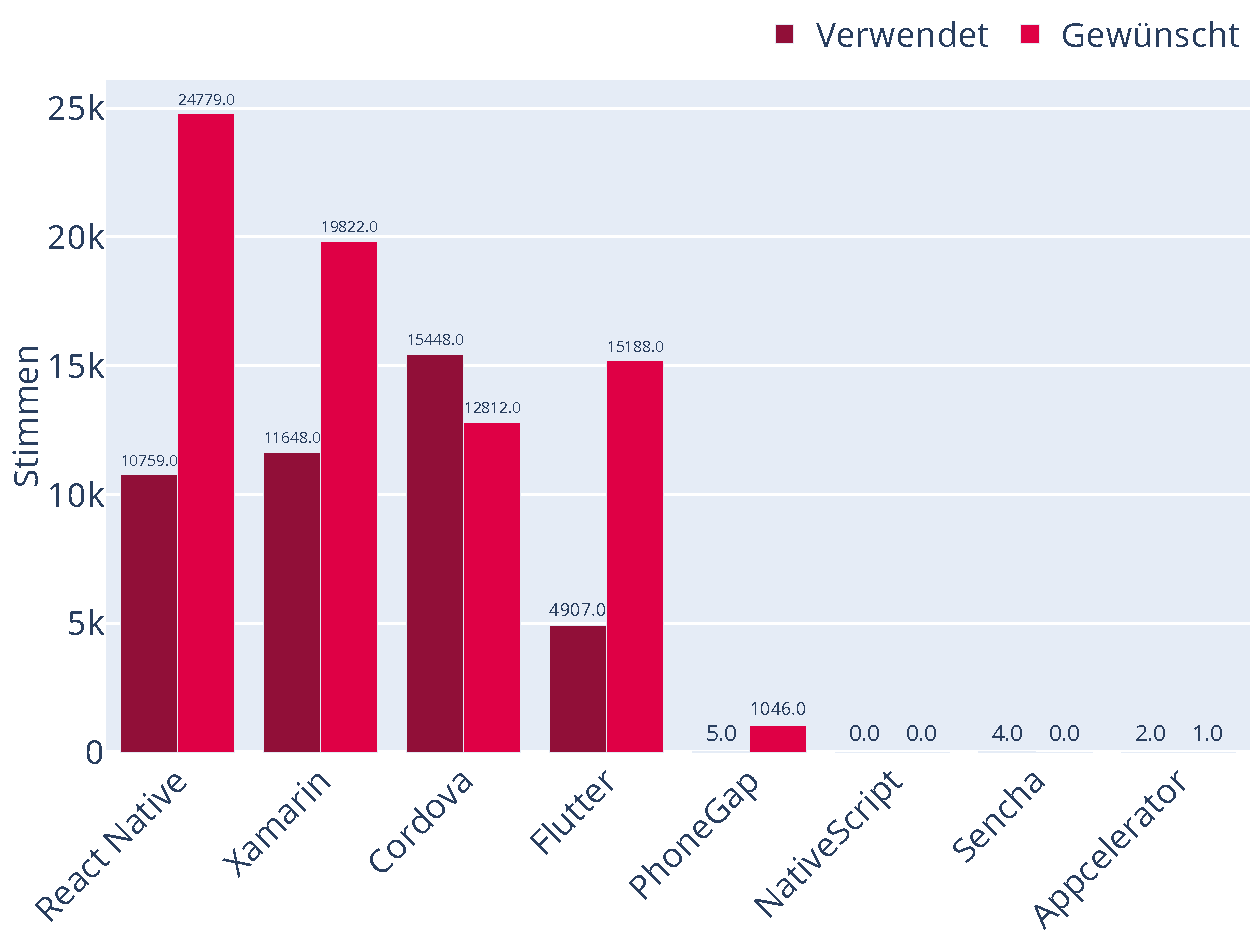
\includegraphics[width=1.0\textwidth]{Charts/Stack Overflow Umfrage/Summe der Stimmen.pdf}
	\caption[Stimmen der Stack Overflow Umfrage von 2013 bis 2020]{Summe der Stimmen der Stack Overflow Umfrage von 2013 bis 2020, Quelle: Eigene Abbildung, Notebook: Charts/Stack Overflow Umfrage/Stack Overflow Umfrage.ipynb}
	\label{fig:SummeDerStimmen}
\end{figure}

Auch das Suchinteresse auf Google ist für diese Frameworks äußerst gering. In Abbildung \ref{fig:SuchinteresseGeringeRelevanz} werden NativeScript, Sencha, Appcelerator und auch Adobe PhoneGap mit Apache Cordova für das relative Suchinteresse verglichen. 

\begin{figure}[H]
	\centering
    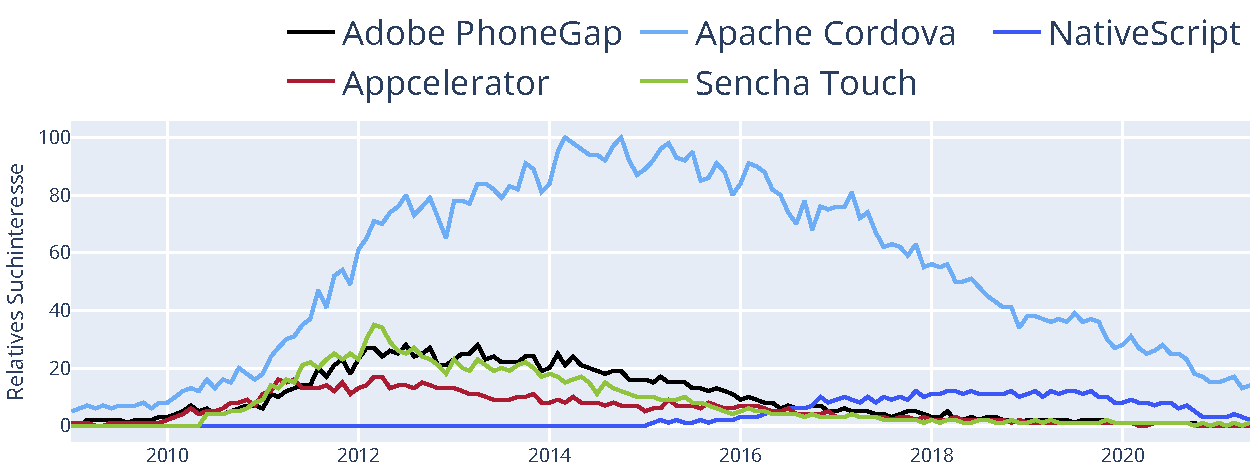
\includegraphics[width=1.0\textwidth]{Charts/Google Trends/Suchinteresse geringe Relevanz.pdf}
	\caption[]{, Quelle: Eigene Abbildung, Notebook: Charts/Google Trends/Google Trends.ipynb, Daten-Quelle: Google Trends\footnote{\cite{FaqPhoneGapDocs}}}
	\label{fig:SuchinteresseGeringeRelevanz}
\end{figure}


\paragraph{Verwandte Technologien zu Apache Cordova} Das Ionic Framework taucht in den Ergebnissen der Stack Overflow Umfragen nicht auf. Ein Grund dafür könnte sein, dass es auf Apache Cordova aufbaut\footnote{\cite{TheLastWordOnCordovaAndPhoneGap}}, welches bereits in den Ergebnissen vorkommt. Adobe PhoneGap taucht zwar in den Ergebnissen von 2013 mit 1043 Stimmen auf (Siehe Abbildung \ref{fig:CordovaUndPhoneGapStimmen}), verliert jedoch in den Folgejahren mit weniger als 10 Stimmen abrubt an Relevanz.  Das stimmt nicht mit dem Suchinteresse auf Google überein, da es dort ab 2013 sogar steigt, wie in Abbildung \ref{fig:SuchinteresseGeringeRelevanz} zu sehen ist. 2013 existierte PhoneGap noch als extra Mehrfachauswahlfeld in den Daten, während es ab 2014 nur noch in dem Feld für die sonstigen Freitext Angaben auftaucht \footnote{Vgl. \cite{StackOverflowInsights}}. Auch Adobe PhoneGap baut auf Apache Cordova auf\footnote{Vgl. \cite{FaqPhoneGapDocs}}. Für diese Auswertung spielen diese verwandten Technologien eine untergeordnete Rolle, da sie auch in den Google Trends weit hinter Apache Cordova zurückbleiben (Abb. \ref{fig:SuchinteresseGeringeRelevanz}).
 
\begin{figure}[H]
	\centering
    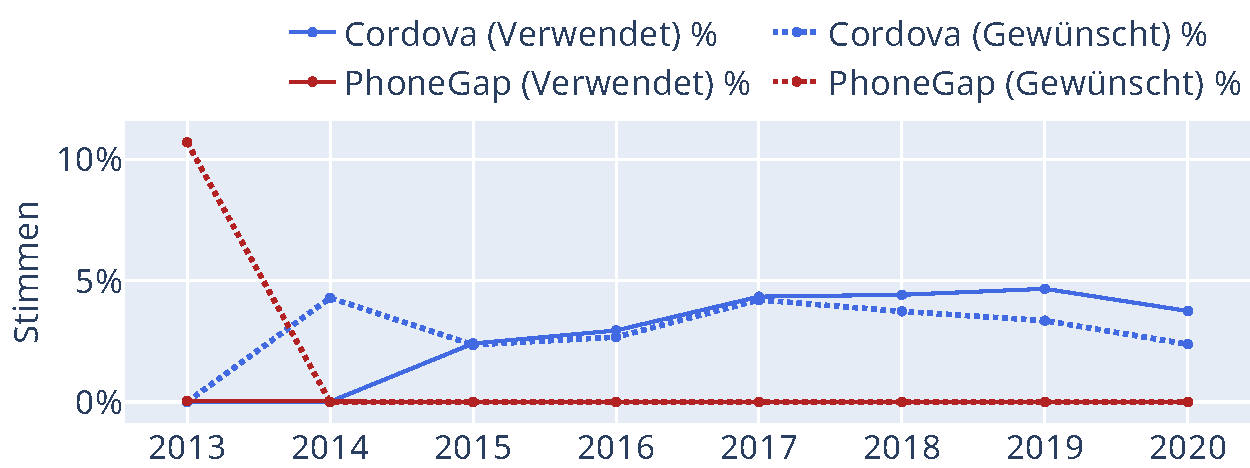
\includegraphics[width=1.0\textwidth]{Charts/Stack Overflow Umfrage/Cordova und PhoneGap Stimmen.pdf}
	\caption[Stimmen für Cordova und PhoneGap 2013 bis 2020]{Stimmen für Cordova und PhoneGap 2013 bis 2020, Quelle: Eigene Abbildung, Notebook: Charts/Stack Overflow Umfrage/Stack Overflow Umfrage.ipynb}
	\label{fig:CordovaUndPhoneGapStimmen}
\end{figure}
 
Am Beispiel von Adobe PhoneGap wird deutlich, wie wichtig es ist, auf eine Technologie zu setzen, die weit verbreitet ist. Im schlimmsten Fall wird die Technologie sogar vom Betreiber aufgrund zu geringer Nutzung komplett eingestellt, wie es bereits bei PhoneGap geschehen ist. Adobe gab am 11. August 2020 bekannt, dass die  Entwicklung an PhoneGap eingestellt wird und empfiehlt die Migration hin zu Apache Cordova.\footnote{Vgl. \cite{UpdateForCustomersUsingPhoneGapAndPhoneGapBuild}}

\subsubsection{Frameworks mit sinkender Relevanz}

Die Technologien Xamarin und Cordova zeigen bereits einen abfallenden Trend, wie in Abbildung \ref{fig:XamarinUndCordovaStimmen} ersichtlich ist. Im Fall von Xamarin gibt es immerhin mehr Entwickler, die sich wünschen, mit dem Framework zu arbeiten, als Entwickler, die tatsächlich mit Xamarin arbeiten. Cordova scheint in diesem Hinblick dagegen eher unbeliebt: es gibt mehr Entwickler, die mit Cordova arbeiten, als tatsächlich damit arbeiten wollen.

\begin{figure}[H]
	\centering
    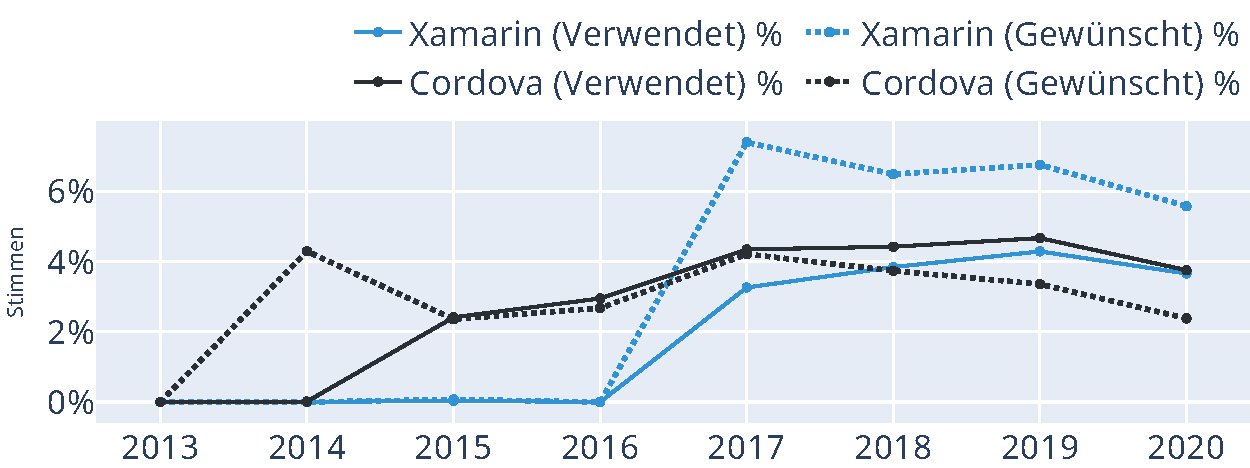
\includegraphics[width=1.0\textwidth]{Charts/Stack Overflow Umfrage/Xamarin und Cordova Stimmen.pdf}
	\caption[Stimmen für Xamarin und Cordova]{Stimmen für Xamarin und Cordova 2013 bis 2020, Quelle: Eigene Abbildung, Notebook: Charts/Stack Overflow Umfrage/Stack Overflow Umfrage.ipynb}
	\label{fig:XamarinUndCordovaStimmen}
\end{figure}

In Abbildung \ref{fig:SuchinteresseSinkendeUndSteigendeRelevanz} ist noch einmal zu sehen, dass Google Trends die Erkenntnisse aus der Stack Overflow Umfrage reflektiert und es wird auch sichtbar, welche beiden Technologien möglicherweise der Grund für den Rückgang von Xamarin und Cordova sind.

\begin{figure}[H]
	\centering
    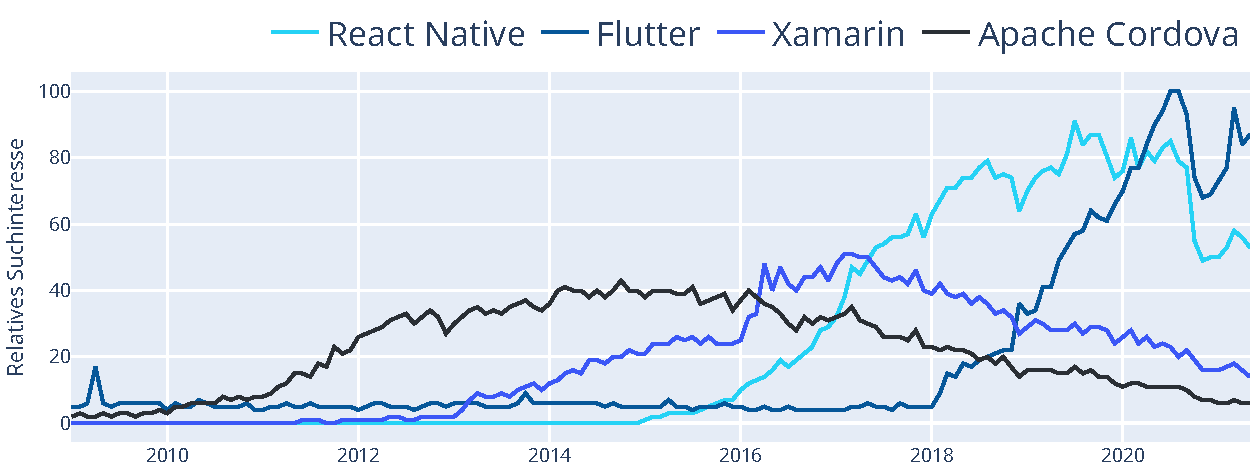
\includegraphics[width=1.0\textwidth]{Charts/Google Trends/Suchinteresse sinkende und steigende Relevanz.pdf}
	\caption[Suchinteresse sinkende und steigende Relevanz]{Suchinteresse sinkende und steigende Relevanz, Quelle: Eigene Abbildung, Notebook: Charts/Stack Overflow Umfrage/Stack Overflow Umfrage.ipynb}
	\label{fig:SuchinteresseSinkendeUndSteigendeRelevanz}
\end{figure}

\subsubsection{Frameworks mit steigender Relevanz}

Besser ist es, auf Technologien zu setzen, die noch einen steigenden Trend der Verbreitung und Beliebtheit zeigen. In Abbildung \ref{fig:ReactNativeUndFlutterStimmen} wird sichtbar, dass es sich dabei um Flutter und immerhin im Hinblick auf die Verbreitung auch für React Native handelt. Ungünstigerweise wird React Native in der Stack Overflow Umfrage erst seit 2018 als tatsächliches Framework abgefragt. Vorher erschien lediglich das Framework React, welches nicht für den Vergleich der Cross-PlatformFrameworks eignet, da es sich um ein reines Web-Framework handelt. Doch auch die Ergebnisse von Google Trends zeigen einen ähnlichen Verlauf für die Jahre 2019 und 2020 (Abb. \ref{fig:SuchinteresseSinkendeUndSteigendeRelevanz}).

\begin{figure}[H]
	\centering
    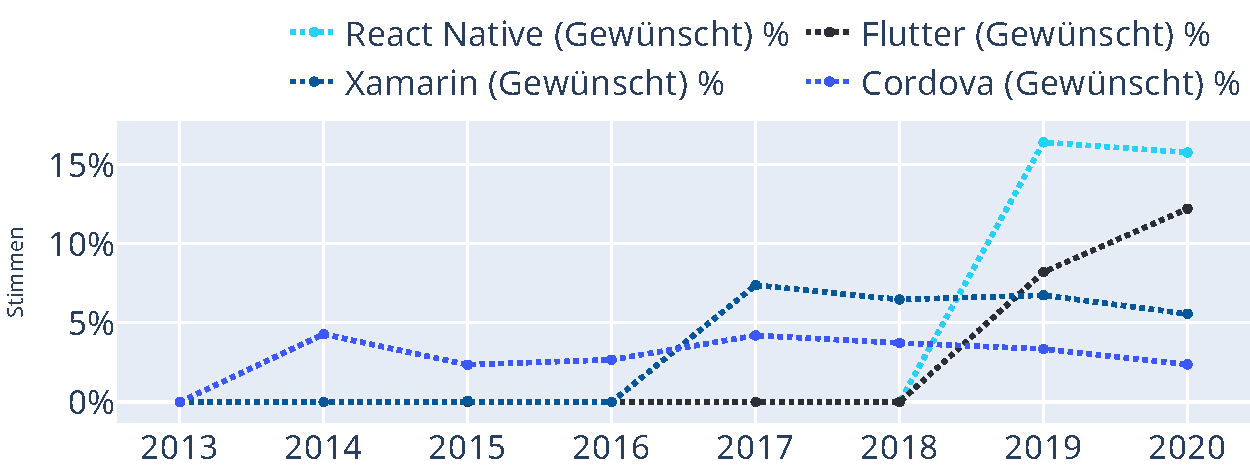
\includegraphics[width=1.0\textwidth]{Charts/Stack Overflow Umfrage/React Native und Flutter Stimmen.pdf}
	\caption[Stimmen für React Native und Flutter]{Stimmen für React Native und Flutter 2013 bis 2020, Quelle: Eigene Abbildung, Notebook: Charts/Stack Overflow Umfrage/Stack Overflow Umfrage.ipynb}
	\label{fig:ReactNativeUndFlutterStimmen}
\end{figure}

Im Vergleich von dem Jahr 2019 mit 2020 wird sichbar, dass die Zahl der Entwickler, die sich wünschen, mit React Native zu arbeiten, gesunken ist. Dennoch ist die Anzahl der Entwickler, die mit React Native arbeiten möchten noch weit höher, als die der Entwickler, die tatsächlich mit React Native arbeiten.

Es ist möglich, dass der abfallende Trend daran liegt, dass die Zahl der Entwickler, die mit Flutter arbeiten möchten im selben Jahr gestiegen ist. React Native hat im Vergleich zu Flutter jedoch noch immer mehr aktive Entwickler und die Tendenz ist steigend. Doch die Anzahl der aktiven Flutter Entwickler zeigt einen noch stärker steigenden Trend. So könnte es sein, dass die Zahl der Flutter Entwickler die der React Native Entwickler in einem der nächsten Jahre überholt. Im Such-Interesse hat sich diese Entwicklung bereits vollzogen (Abb. \ref{fig:SuchinteresseSinkendeUndSteigendeRelevanz}).

Nichtsdestotrotz scheinen beide Technologien als Kandidaten für einen detaillierteren Vergleich für dieses Projekt in Frage zu kommen. Im nächsten Kapitel soll evaluiert werden, welches Framework für die Entwicklung der Formular-Anwendung angemessener ist.



